\section{Pulse Processing Electronics}
\subsection{General Concepts}
\begin{itemize}
    \item In the context of this course, signal amplification and shaping is done in analog then converted to digital  
    \item As shown in figure~\ref{fig:signal_processing}, the signal processing and pulse-shape system goes as the following:\\
    An incident radiation interacts in the detector and deposits energy as a current pulse that is usually too small to be measured directly. The current is therefore sent to the preamplifier, which integrates the transient current pulse to produce a voltage step that is proportional to the pulse. The shaping amplifier then converts the output of the preamplifier into a form suitable for measurements, producing an output voltage pulse with its pulse height proportional to the initial deposited charge. 
\end{itemize}
\begin{figure}[ht]
    \centering
    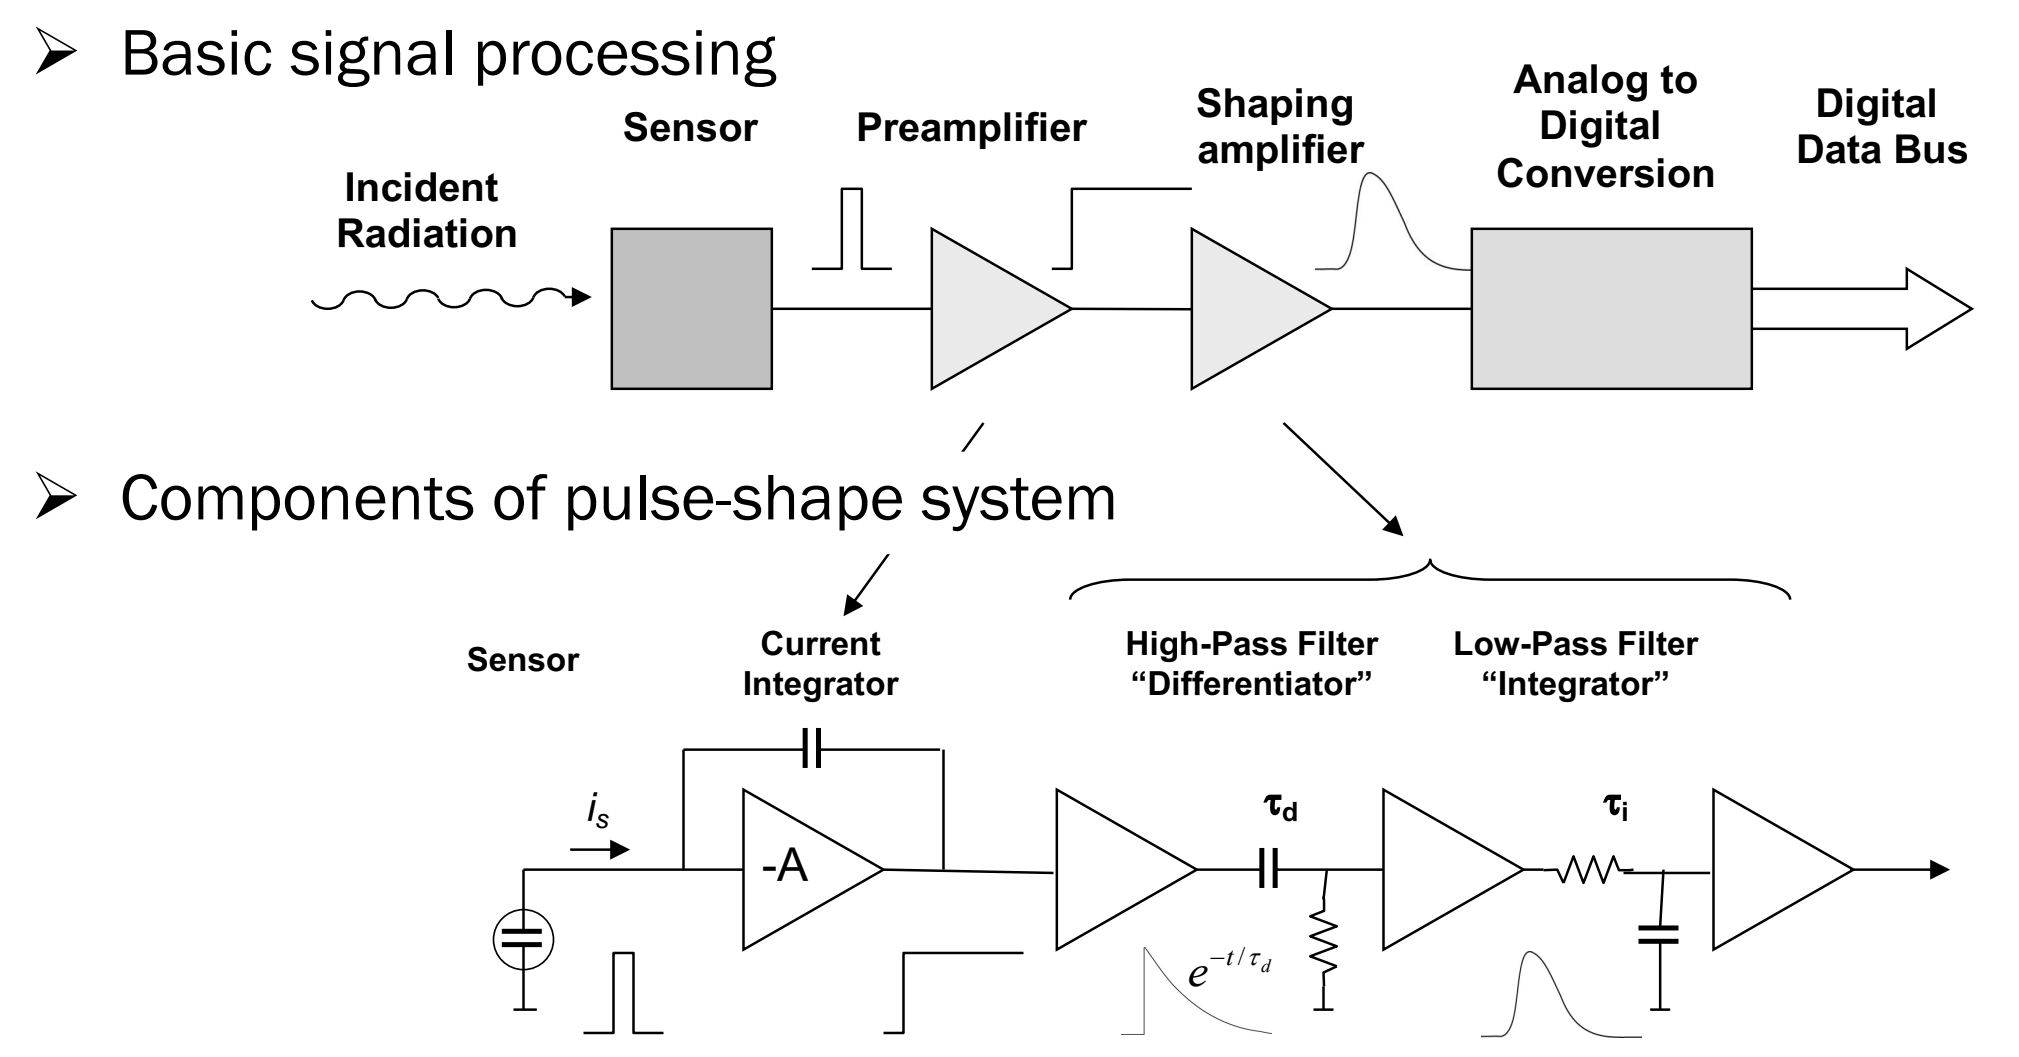
\includegraphics[width=0.8\textwidth]{images/signal_processing_diagram.png}
    \caption{Signal processing diagram.}
    \label{fig:signal_processing}
\end{figure}
\subsection{Components}
\subsubsection{Preamplifier}
\begin{figure}[ht]
    \centering
    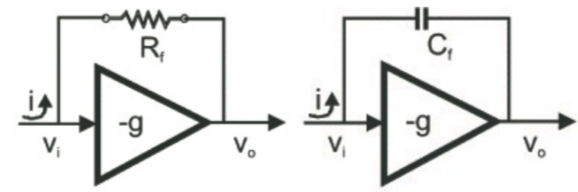
\includegraphics[width=0.45\textwidth]{images/preamp_circuit_current_charge.png}
    \caption{Circuits of the current (left) and charge (right) sensitive preamplifiers.}
    \label{fig:preamp_circuit_current_charge}
\end{figure}
\begin{figure}[ht]
    \centering
    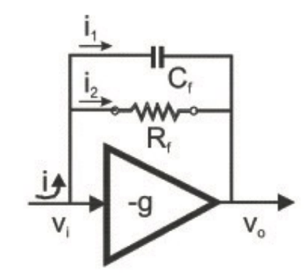
\includegraphics[width=0.25\textwidth]{images/preamp_circuit_resistive_feedback.png}
    \caption{Circuit of the resistive feedback preamplifier.}
    \label{fig:preamp_circuit_resistive_feedback}
\end{figure}
\begin{enumerate}
    \item General function:
    \begin{itemize}
        \item Convert charge to voltage
        \item Amplifies a signal with minimal noise
        \item Matches the high detector impedance to the low impedance of amplifier input
        \item Filters very low frequencies
    \end{itemize}
    \item Current-sensitive preamplifier, see figure~\ref{fig:preamp_circuit_current_charge} (left):
    \begin{itemize}
        \item[] The op-amp gives $V_o=-gV_i$
        \item[] $iR_f=V_i-V_o$
        \item[] $V_o-\frac{iR_f}{1+1/g}\approx-iR_f$
    \end{itemize}
    \item Charge-sensitive preamplifier, see figure~\ref{fig:preamp_circuit_current_charge} (right):
    \begin{itemize}
        \item[] $q=\int_0^ti\;dt'=C_f(V_i-V_o)$
        \item[] $V_o=-\frac{q}{C_f(1+1/g)}\approx-\frac{q}{C_f}$
    \end{itemize}
    \item Resistive feedback preamplifier, see figure~\ref{fig:preamp_circuit_resistive_feedback}:
    \begin{itemize}
        \item[] $V_i-V_o=-V_o(1+1/g)=\int_0^t\frac{i_1}{C_f}dt'=i_2R_f$
        \item[] $i=i_1+i_2=-C_f(1+1/g)\frac{dV_o}{dt}-(1+1/g)V_o/R_f$
        \item[] $\Rightarrow\; \frac{dV_o}{dt}+\frac{1}{\tau}V_o=\frac{-i}{C_f(1+1/g)}$ , $\tau=R_fC_f$
        \item[] $\Rightarrow$ For $i(t')=-q\delta(t')$, $V_0=-\frac{qe^{-t/\tau}}{C_f(1+1/g)}$ , $\tau\gg t_\text{collection}$
        \item These preamplifiers are limited by pile-up and additional noise due to $R_f$; an alternative would be pulsed-reset preamplifiers.
        \item Preamplifier gain is given by $V_{out}/q_{in}$, in units of $[V/pC]$;\\
        $V_{out}$ is measured at the peak of the pulse.
    \end{itemize}
\end{enumerate}
\subsubsection{Shaping or Linear Amplifier}
\begin{enumerate}
    \item General function:
    \begin{itemize}
        \item Increases the amplitude of the signal to a convenient voltage for a discriminator, pulse-height analyze, or other pulse-processing units
        \item Shapes the signal by filtering high and low frequency noise and shortens the long pulse tail to avoid pile-up
    \end{itemize}
    \item Pulse-processing
    \begin{enumerate}
        \item CR circuit (differentiator, HPF), see figure~\ref{fig:RC_CR_circuits} (left):
        \begin{itemize}
            \item[] $V_{in}=Q/C+V_{out}$
            \item[] $\frac{dV_{in}}{dt}=\frac{1}{C}\frac{dQ}{dt}+\frac{dV_{out}}{dt}$
            \item[] With $i=\frac{dQ}{dt}=\frac{V_{out}}{R}$ and $\tau=RC$
            \item[] $V_{out}+\tau\frac{dV_{out}}{dt}=\tau\frac{dV_{in}}{dt}$
            \item For small $\tau$ (fast electronics), $V_{out}\approx\tau\frac{dV_{in}}{dt}$\\
            The differentiator removes low frequency components and is called a high-pass filter.
            \item For large $\tau$ (slow electronics), $\tau\frac{dV_{out}}{dt}\approx\tau\frac{dV_{in}}{dt}$, $V_{out}\approx V_{in}$
        \end{itemize}
        \item RC circuit (integrator, LPF), see figure~\ref{fig:RC_CR_circuits} (right):
        \begin{itemize}
            \item[] $V_{in}=iR+V_{out}$
            \item[] With $i=\frac{dQ}{dt}=C\frac{V_{out}}{dt}$ and $\tau=RC$
            \item[] $V_{in}=\tau\frac{dV_{out}}{dt}+V_{out}$
            \item For small $\tau$ (fast electronics), $V_{out}\approx V_{in}$
            \item For large $\tau$ (slow electronics), $\frac{V_{in}}{\tau}\approx \frac{dV_{out}}{dt}\;\Rightarrow\;\frac{1}{\tau}\int V_{in}dt\approx V_{out}$\\
            The integrator removes high frequency components and is called a low-pass filter.
        \end{itemize}
    \end{enumerate} 
\end{enumerate}
\begin{figure}[ht]
    \centering
    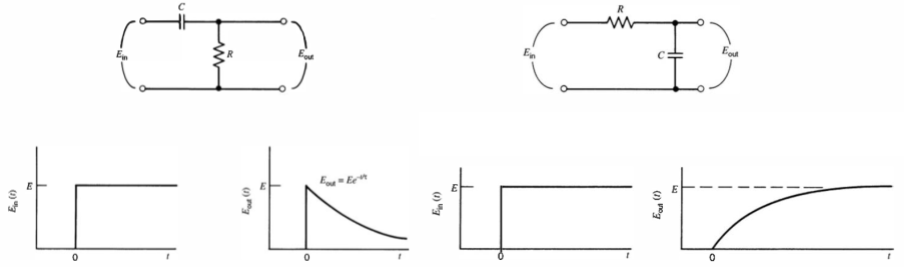
\includegraphics[width=1.0\textwidth]{images/RC_CR_circuits.png}
    \caption{The CR (left) and RC (right) circuits.}
    \label{fig:RC_CR_circuits}
\end{figure}
\subsection{Measurements of Interest}
\subsubsection{Energy Measurement}
\begin{itemize}
    \item General concept
    \begin{itemize}
        \item Assuming voltage amplitude to be proportional to energy deposition in a detector, we would like to determine the amplitude as accurately as possible
        \item Uncertainties arise from 
        \begin{itemize}
            \item[(a)] Noise from the detector, readout, and electronics
            \item[(b)] The charge creation and collection process, which are energy and position dependant
            \item[(c)] Electronics ``drift''
        \end{itemize}
        \item To achieve accuracy, we filter/ perform shaping of the preamplifier output signals to reduce noise without attenuating important signal features
        \item Filtering can either be done in the analog domain (e.g., with a CR-(RC)$^n$ filter) or in the digital domain (e.g., with a trapezoidal filter)
    \end{itemize}
    \item Electronic noise\\
    See figure~\ref{fig:log_noise}.
    \begin{enumerate}
        \item Series (voltage) noise:\\
        Johnson noise (intrinsic noise from Brownian thermal motion) associated with series resistance and thermal noise of the input FET in the detection system. 
        \item Parallel (current) noise:\\
        Fluctuations in the surface and bulk leakage currents
        \item 1/f noise:\\
        Capture and release of charges in the input FET, independent of frequency and shaping time.
    \end{enumerate}
    \begin{figure}[ht]
        \centering
        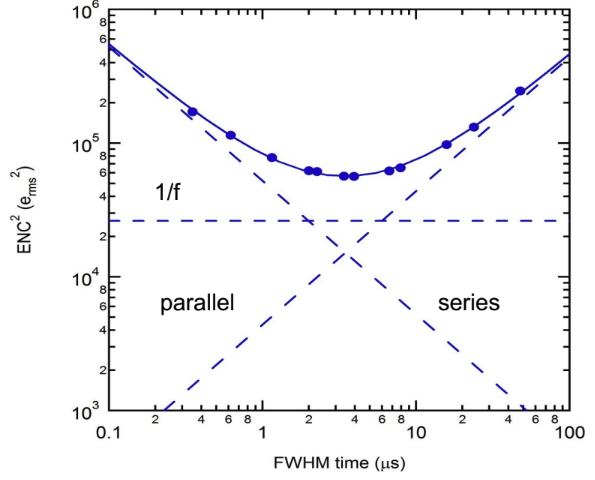
\includegraphics[width=0.4\textwidth]{images/log_noise.png}
        \caption{Noise vs. shaping time plot. ENC stands for equivalent noise charge.}
        \label{fig:log_noise}
    \end{figure}
    \item CR-(RC)$^n$ shaping
    \begin{itemize}
        \item By adding several RC circuits after CR circuits, the signal-to-noise ratio can be optimized (e.g., approximate Gaussian shaping). Typically, $\tau_{CR}=\tau_{RC}$ .
        \item Since the preamplifier output signal is not a step function but has finite decay time, the RC-CR generally creates an undershoot in the amplifier output. This can be compensated by pole-zero cancellation. 
        \item To avoid pile-up, one would generally like to keep shaping times short so that the shaped waveform can return to the baseline as quickly as possible.
        \item However, only by keeping the shaping time long compared to the charge collection time in the detector, can we avoid ballistic deficits. Ballistic deficits are caused by variations in rise-time, possibly due to position-dependent charge collection behavior. For these types of detectors, pulse shaping methods that lead to a shaped pulse with a flat top (e.g. trapezoidal shaping) would be favored. 
    \end{itemize}
\end{itemize}
\subsubsection{Time Measurement}
\begin{itemize}
    \item General concepts:
    \begin{itemize}
        \item To determine arrival time of radiation
        \item There are three types of uncertainties (see figure~\ref{fig:time_measurement_unc}):
        \begin{itemize}
            \item[(a)] Detector-intrinsic signal rise time (response time)
            \item[(b)] Jitter: Variations with fixed amplitude (noise)
            \item[(c)] Walk: Variations in signals and in rise times (position and energy dependant)
        \end{itemize}
        \item Mostly based on trigger-level crossing resulting in a logic pulse whose time reflects the arrival time
    \end{itemize}
    \begin{figure}[ht]
        \centering
        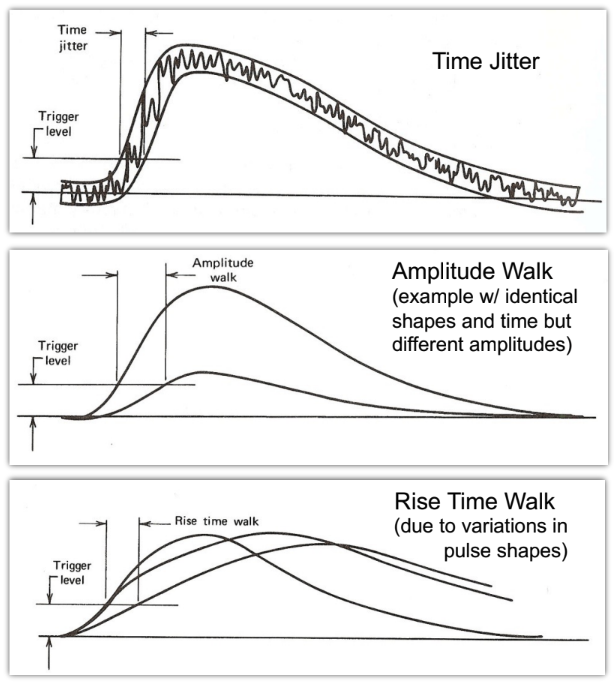
\includegraphics[width=0.4\textwidth]{images/time_measurement_unc.png}
        \caption{Various types of uncertainties in time measurements.}
        \label{fig:time_measurement_unc}
    \end{figure}
    \item Leading edge triggering
    \begin{itemize}
        \item Shown in figure~\ref{fig:time_measurement_unc}, it is the simplest and most direct time pick-off method.
        \item Time is determined to be when the signal crosses a fixed discriminator threshold (leading edge discriminator).
        \item A low threshold would minimize walk, a high threshold at steepest slope of the signal would minimize jitter.
    \end{itemize}
    \begin{figure}[ht]
        \centering
        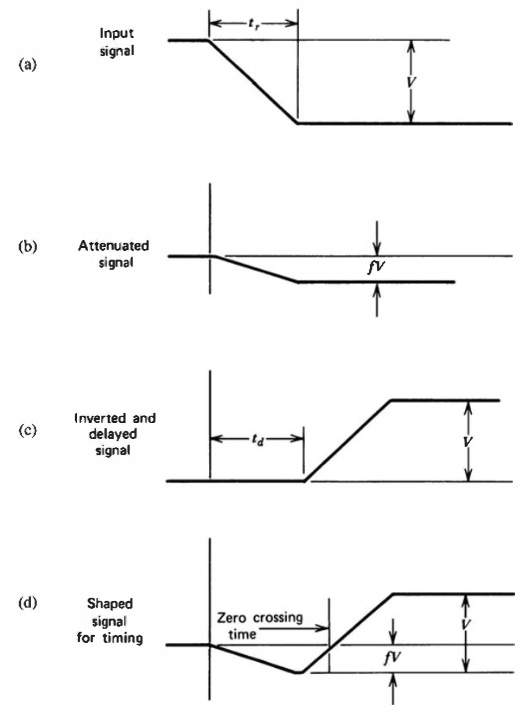
\includegraphics[width=0.5\textwidth]{images/constant_fraction_discriminator.png}
        \caption{The constant fraction time pick-off method.}
        \label{fig:constant_fraction_discriminator}
    \end{figure}
    \item Constant fraction discriminator
    \begin{itemize}
        \item An enhancement of leading edge triggering, see figure~\ref{fig:constant_fraction_discriminator} for its time pick-off method. 
        \item The threshold is a constant fraction of the signal amplitude; time pick-off is independent of walk.
        \item For semiconductor detectors, $f\approx0.2$ and $t_d\approx50\;ns$. (See figure~\ref{fig:constant_fraction_discriminator} for definitions of $f$ and $t_d$.)
    \end{itemize}
    \item Implementation
    \begin{itemize}
        \item Multichannel time spectroscopy (prompt and chance coincidence spectra): \\
        The simplified setup and the corresponding time spectrum is shown in figure~\ref{fig:prompt_and_chance_coincidence}.
        \item Assuming that the isotope emits at least two radiations in true coincidence, these true coincidence events will appear in the same region of the time spectrum, producing a prompt coincidence peak. 
        \item Without the fixed delay, we would only be able to see half of the peak (since it would be centered at 0). The width of the peak is decided by the walk and jitters of the system. 
    \end{itemize}
    \begin{figure}[ht]
        \centering
        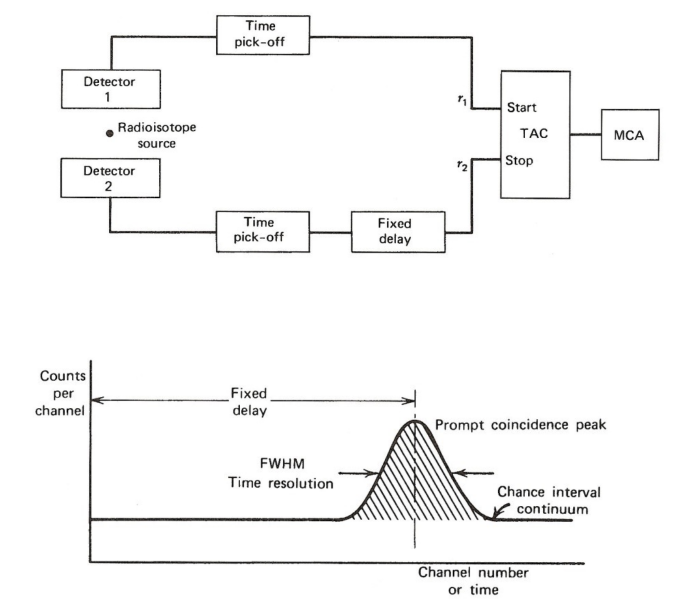
\includegraphics[width=0.7\textwidth]{images/prompt_and_chance_coincidence.png}
        \caption{Multichannel time spectroscopy using coincidence radiation. TAC stands for ``time-to-amplitude converter'', which produces an output pulse with an amplitude proportional to the time interval between input ``start'' and ``stop'' pulses.}
        \label{fig:prompt_and_chance_coincidence}
    \end{figure}
\end{itemize}
\subsection{Other Components}
\begin{itemize}
    \item Coaxial cables
    \begin{itemize}
        \item Cables should be terminated with load $R$ equal to the impedence of the cable; an open cable results in positive reflection, and a shorted cable results in negative reflection.
    \end{itemize}
    \item Pulse attenuators and splitters
    \item Pulse generators
    \item For spectrum enhancement:
    \begin{itemize}
        \item Pulse-shape discrimination
        \item Pile-up rejection
        \item Baseline restoring
        \item SCA (single-channel analyzers)
        \item MCA (multi-channel analyzers)
        \item Coincidence units
        \item TAC
    \end{itemize}
\end{itemize}
